\title{Babascript: }

\etitle{Babascript: }

\author{匿名で査読を行うため著者名なし
  \affil{匿名で査読を行うため所属名なし}}

\begin{abstract}

プログラムはコンピュータを制御できるが、人は制御できない。
人をプログラムから制御できれば、コンピュータのみでは実現出来なかった処理も実現可能となる。
そこで、本論文では、プログラムに人への処理命令を組み込むことのできるプログラミング環境 Babascript を提案する。
Babascriptでは、人とコンピュータはプログラム上で対等な処理ノードとなり、相互補完的に動作することで
また、Babascriptフレームワークによって実現する応用例を示し、起こりうる問題について考察する。

\end{abstract}

\maketitle

\section{はじめに}\label{ux306fux3058ux3081ux306b}

プログラムはコンピュータを制御できるが、人を制御することはできない。
既存のプログラムの仕様には、人に対する制御命令構文が存在するものはなく、
コンピュータを制御するためのものである。

人はコンピュータに比べ、とても柔軟な能力を有する。
単純な演算能力や記憶能力だけで言えば、コンピュータのほうが優れていることもあるが、
場の空気を読んだり、人とのコミュニケーションは人のほうが得意であると言える。

人は、コンピュータにはない貴重な能力を有しており、プログラムにとっても有用である。
しかし、人をプログラムから制御出来るような仕組みの研究はクラウドソーシングの分野に限られている。
クラウドソーシングはインターネットを介した不特定多数の人をリソースとして扱うものであり、
利用可能な能力は限られている。 また、専用の記法を利用する必要があった。
不特定な人ではなく、特定の人をプログラムから操作できるようになれば、
プログラムが干渉可能な領域は更に広がると考えられる。

そこで、本論文では、Babascriptプログラミング環境を提案する。
Babascriptプログラミング環境は、関数呼び出しによって人に処理命令の通知ができるDSL
Babascrtipt(図\ref{script_01})と、
Babascriptからの命令を受け取り、処理結果を入力することのできるクライアントライブラリ(図\ref{client})及び
スマートフォンアプリケーションのBabascript
Client(図\ref{webapp-interface})から構成される。

\begin{figure}[h]
  \centering
  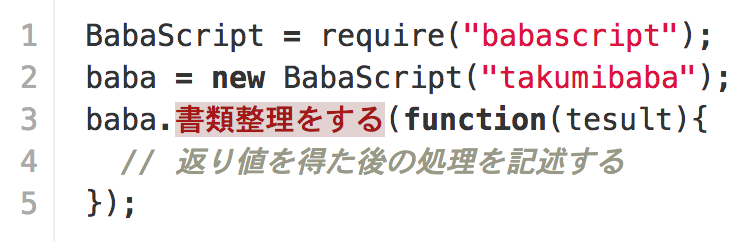
\includegraphics[width=220px]{./images/script_01.png}
  \caption{babascriptプログラムの基本命令文}
  \label{script_01}
\end{figure}

\begin{figure}[h]
  \centering
  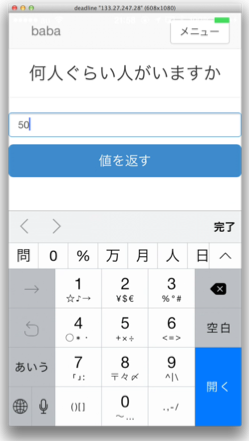
\includegraphics[width=120px]{./images/interface.png}
  \caption{Webアプリのインタフェース}
  \label{webapp-interface}
\end{figure}

Babascriptを利用することで、通常のプログラムと人への処理命令をほぼ同じ記述で実現することができる。
これによって、特別な記法の知識が必要なく、
既存のプログラムの書き方人の力を借りたプログラミングが可能となる。

コンピュータと人が従順な処理ノードとして、プログラムからの命令を積極的に処理していくことによって、
相互補完しながら全体の処理を最適化できると考えられる。
つまり、コンピュータはその演算能力を最大限に活かし人を助け、
人はその柔軟な思考力や実世界への干渉力を活かしてコンピュータにはできない処理を実現する。
こういった仕組みによって、人にとっての処理の最適化を狙う。
また、その例として「仕事のプログラム化」と「人力実世界プログラミング」を示す。

\section{BabaScript}\label{babascript}

Babascriptは、関数呼び出しによって人に処理命令を送れるオブジェクト(以下、人オブジェクト)を宣言可能にするDSLである。
人オブジェクトにおいて定義されていない全てのメソッドが人への命令(以下、人への命令構文)として解釈され、人に通知される。
また、人からの返り値を得ると、人への命令構文の引数で指定したコールバック関数を実行する。

\subsection{人オブジェクトの宣言と処理命令構文}\label{ux4ebaux30aaux30d6ux30b8ux30a7ux30afux30c8ux306eux5ba3ux8a00ux3068ux51e6ux7406ux547dux4ee4ux69cbux6587}

図\ref{script_01}のようなプログラムによって、人に処理命令を送ることができる。
人への命令構文は実行後、メソッド名と引数を元にしたjsonオブジェクトを生成する。
生成されたjsonオブジェクトは、命令としてクライアントライブラリに配信される。
この際、オブジェクトに定義されいない全てのメソッドが人への命令構文として解釈される。
この機能はmethodmissingと呼ばれる、定義されていないメソッドが実行された際の処理を記述しておくと、その処理を実行する機能によって実現している。

人オブジェクトは宣言時にIDを指定することによって、誰に対して命令を配信するかを決定する。
例えば、id:baba
に命令を送りたければ、人オブジェクト宣言時の第一引数にはbabaという文字列を指定する必要がある。
また、クライアント側でも同様に、id:baba として宣言する必要がある。

この際、指定したIDを監視するクライアントが複数人だった場合は、後述するbroadcastオプションをつかってない場合は、
命令を実行していないクライアントへと順番に配信される。

人への処理命令構文の第一引数にはクライアント側に送信するオプション情報を指定し、
第二引数には返り値が得られた際に実行するコールバック関数を指定する。
コールバック関数実行時には、その引数に返り値と命令情報、実行者情報を格納したオブジェクトが与えられる。

\subsection{オプション情報の付加}\label{ux30aaux30d7ux30b7ux30e7ux30f3ux60c5ux5831ux306eux4ed8ux52a0}

人への処理命令構文の第一引数に与えるオプション情報には、返り値の型指定などの情報が考えられる。
例えばBoolean型を指定する場合には図\ref{script_02}のようなプログラムが考えられる。
他にも、指定したリストの中から値を選択してほしい、といった命令の場合は、リスト情報を格納した配列を指定する。
このオプション情報の処理は基本機能には含まれていないため、ライブラリを利用して実装する応用アプリケーションごとに対応する必要がある。

\begin{figure}[h]
  \centering  
  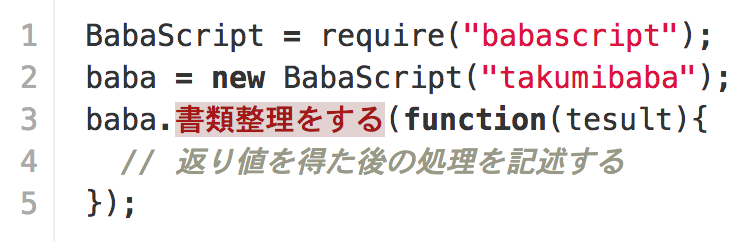
\includegraphics[width=220px]{./images/script_02.png}
  \caption{オプション情報}
  \label{script_02}
\end{figure}

特別なオプション情報として、broadcastオプションが存在する。
broadcast機能は、指定したIDを監視する全てのクライアントへとタスクを配信し、指定した数の返り値を得られると処理を終了し、コールバック関数を実行するといったものだ。

\subsection{サンプルコード}\label{ux30b5ux30f3ux30d7ux30ebux30b3ux30fcux30c9}

以下にサンプルコードを示す。

\begin{figure}[h]
  \centering  
  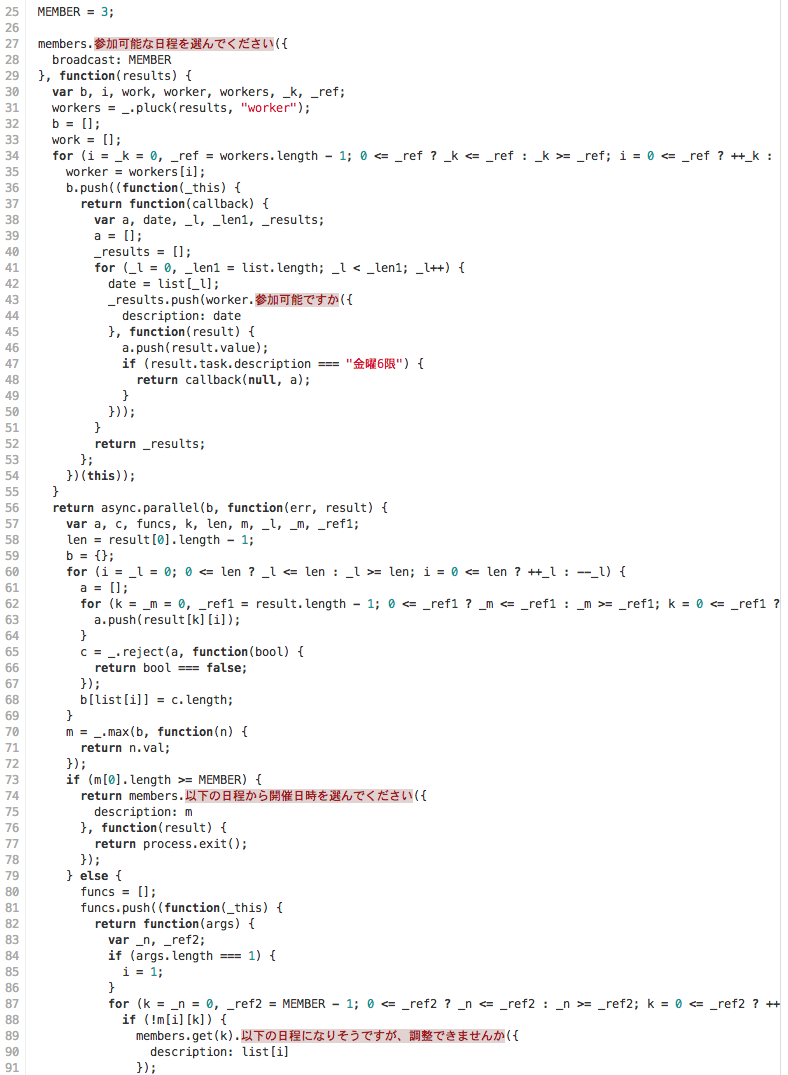
\includegraphics[width=220px]{./images/samplecode.png}
  \caption{サンプルコード}
  \label{script_02}
\end{figure}

\subsection{Babasciript Client}\label{babasciript-client}

Babascript
Clientは、Babascriptからの命令受信と処理結果の送信機能を実現するクライアントライブラリだ。
命令受信のイベントに対してコールバック関数を指定することで、処理命令を受け取ることができる。
基本的な利用方法は、図\ref{client}に示す。

\begin{figure}[h]
  \centering
  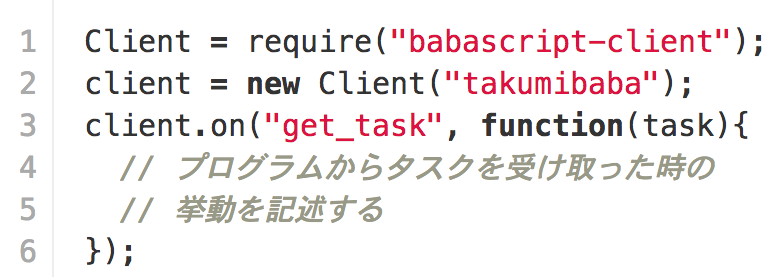
\includegraphics[width=220px]{./images/client.png}
  \caption{クライアントライブラリの基本機能 }
  \label{client}
\end{figure}

クライアントオブジェクトの宣言時、IDを指定することによって、IDに対して処理命令が発行された際にタスクを受信することができる。
また、クライアントオブジェクトが持つreturnValueメソッドを利用することで、返り値を命令発行元に返すことができる。

クライアントライブラリは、UIと完全に分離した実装となっており、かつ利用方もシンプルだ。
後述のWebアプリケーションだけでなく、様々なアプリケーションに組み込むことができる。

\subsection{Webアプリケーション}\label{webux30a2ux30d7ux30eaux30b1ux30fcux30b7ux30e7ux30f3}

BabascriptClientが得たタスクをユーザに提示するためのインタフェースとして、Webアプリケーションを実装した。
タスク情報において型指定をすることによって、ユーザに提示するUIを変化させ、型に合った返り値を選択できるようにしている。
例えば、Boolean型を指定していた場合、ユーザには true ボタンと false
ボタンが提示され、どちらかを押すと、その結果が返り値としてプログラムに返される。

スマートフォンに最適化したWebアプリケーションとして実装しており、様々な場面において利用可能であり、実世界におけるタスクを処理しながらでも十分に利用可能である。
図\ref{webapp-interface}のような画面を持つ。

\section{実装}\label{ux5b9fux88c5}

上記システムは全てJavascriptで実装した。 Babascript
はNode.js上で動作し、 Babascript
ClientはNode.jsとWebブラウザ上で動作する。
全体図は図\ref{system}のとおりだ。

\begin{figure}[h]
  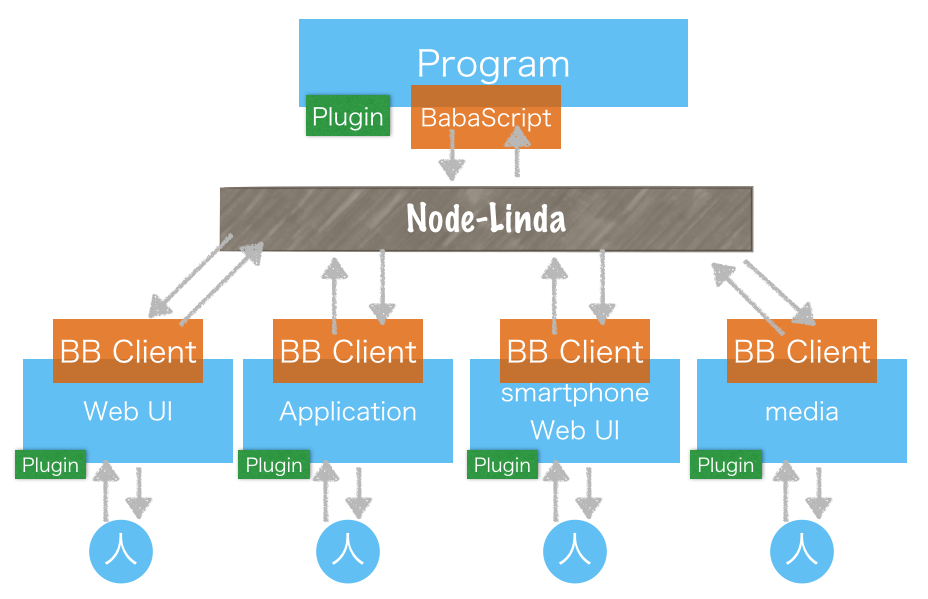
\includegraphics[width=220px]{./images/system.png}
  \caption{システム全体図}  
  \label{system}
\end{figure}

\subsection{処理の流れ}\label{ux51e6ux7406ux306eux6d41ux308c}

Babascript環境は、以下のようなフローで一回の人への命令構文が実行される。

\begin{enumerate}
\def\labelenumi{\arabic{enumi}.}
\itemsep1pt\parskip0pt\parsep0pt
\item
  人への命令構文を実行する
\item
  命令構文の内容に基づき、タスクが生成される
\item
  タスクがNode-Lindaサーバを経由してクライアントへと配信される
\item
  タスクを受け取ったクライアントがユーザに処理を促す
\item
  タスク実行者が、処理結果を入力する
\item
  処理結果を元に返り値データが生成される
\item
  Node-Lindaサーバを経由して実行元プログラムに返り値が送信される
\item
  指定されたコールバック関数が実行され、処理が続く
\end{enumerate}

\subsection{タスク情報の構成}\label{ux30bfux30b9ux30afux60c5ux5831ux306eux69cbux6210}

人への処理命令構文の実行によってタスク情報が生成される。
このタスク情報は、図\ref{task}のようなjsonオブジェクトとなる。

\begin{figure}[h]
  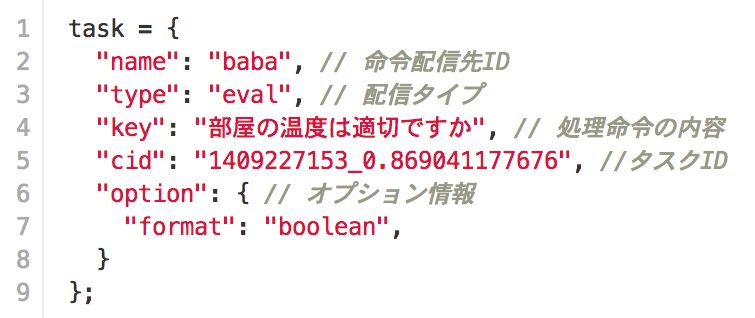
\includegraphics[width=230px]{./images/task.png}
  \caption{タスクのJSONオブジェクト}  
  \label{task}
\end{figure}

\subsection{実行結果の待ち方}\label{ux5b9fux884cux7d50ux679cux306eux5f85ux3061ux65b9}

人への命令構文に対する返り値が、適切に返り値として戻されるようにするために、命令ごとにユニークなIDを生成している。
ユニークIDは、人への命令構文実行時のUNIX time
と、ランダムな数値を結合した文字列である。
図\ref{task}におけるjsonオブジェクトの'cid'の項目に示されているものだ。
このユニークIDは人への命令構文実行時に生成され、ユニークIDを
このユニークIDを伴った返り値が戻ってくるか、指定したタイムアウト時間に到達するか、タスクキャンセルが発生するまで、

\subsection{script-client間の通信}\label{script-clientux9593ux306eux901aux4fe1}

scriptとclientのタスク送受信のために、node-linda\cite{linda}を利用した。
script,
client共に、このnode-lindaに接続するためのライブラリを組み込んでいる。

scriptは、プログラム実行時にnode-lindaサーバに接続し、人への命令構文を実行するごとに、タスクをnode-lindaサーバに書き込む。
書き込み終了後、そのタスクと同じIDを持った返り値タスクが書き込まれるまで、node-lindaサーバの監視を行う。

clientは、プログラム起動中は常にnode-lindaサーバに接続し、指定したIDを監視し、タスク受信まで待機する。
node-lindaサーバに同一IDにタスク書き込みが行われた際、そのタスクを取得する。
このタスクは、broadcastオプションが付いている場合は、同一IDを監視している全てのクライアントがタスクを受信する。
通常の実行の場合は、キューの最初のクライアントのみがタスクを受信・実行し、他のクライアントは待機を継続する。
clientは、タスク実行中は通常のタスクを受信することはなく、タスク実行が終わって受信待ち状態になる際に新たにキューに追加される。
このため、複数のクライアントが一つIDを監視している状況であっても、一つのクライアントにタスクが集中するといったことはない。

\section{応用例}\label{ux5fdcux7528ux4f8b}

以下のような応用が考えられる。

\subsection{仕事のプログラム化}\label{ux4ed5ux4e8bux306eux30d7ux30edux30b0ux30e9ux30e0ux5316}

人への行動命令がプログラムとして記述可能になることで、人の仕事をプログラム化することができる。
プログラム化し、実行することによって、状態をプログラムによって管理することが可能となる。
つまり、条件判断や記憶が必要なことは出来るだけコンピュータ側に処理させる、といったことが可能になり、人は細かい条件などを覚えておいたり、自分で判断することなく、ただ指示されたことのみを実行することで、仕事を終わらせることができるようになる。
ただ指示されたことのみを実行するだけで良いならば、仕事の引き継ぎなども必要なくなり、人の代替も容易となる。

また、人同士がコミュニケーションを取ることなく、複数人を協調させるといったことも可能となる。
通常、複数人を協調させるためには、人同士が相談したり、上位の意思決定者が必要となる。
しかし、コミュニケーションはコストのかかるものであり、適切に行われない場合、問題が生じることもある。
意思決定をプログラムに委ねることは、複数人を効率よく協調させることに繋がるとも考えられる。

全ての仕事をプログラム経由にすることで、詳細な実行ログや実行状況を把握することもできる。
仕事の実行量の定量化や、状況監視、状況の可視化などに活かすことができる。

\subsection{人力実世界プログラミング}\label{ux4ebaux529bux5b9fux4e16ux754cux30d7ux30edux30b0ux30e9ux30dfux30f3ux30b0}

人をセンサーやアクチュエータとして利用することで、人によって実世界を操作する実世界プログラミングが可能となる。
現在のセンサーやアクチュエータでは、実世界に干渉するのには限界がある。
例えば、その場の雰囲気を数値化したり文字列化するといった、コンテキスト情報を伴ったセンシングは困難である。
人というセンサーをプログラムから利用できるようにすることで、今までには実現しなかった処理が実現する。

\section{考察}\label{ux8003ux5bdf}

Babascript環境について、以下のように考察する。

\subsection{処理単位としての人}\label{ux51e6ux7406ux5358ux4f4dux3068ux3057ux3066ux306eux4eba}

本研究では、人は処理を命令され実行するノードとなり、プログラム上においてコンピュータやセンサーと同等となる。
こういったことに対して心理的な拒否感を覚えることも考えられる。
しかし、一処理ノードとして扱うことによって、大きなメリットもある。
人とコンピュータ、処理に応じて適切なほうに実行させることができれば、人は人にしかできないことや人がやるべき処理にのみ集中するといったことも実現できる。
また、ただやるべきことのみを命令されて動くということは、自分で深く考えて行動する必要がないということだ。
とても楽なことでもある。

\subsection{タスク実行の遅延と実行保障性}\label{ux30bfux30b9ux30afux5b9fux884cux306eux9045ux5ef6ux3068ux5b9fux884cux4fddux969cux6027}

Babascriptによってタスク実行を依頼しても、人がすぐにタスクを実行し値を返すことを完全に保証することはできない。
タスク受信端末を見ていない、受信しても実行できないといった状況の場合、すぐに値を返すことはできない。
この際、Babascriptによる処理が原因で全体の処理が遅延する可能性がある。

また、労働関係にあるなど、タスク実行に強制力がある場合は、タスク実行が確実に行われると考えられるが、強制力がない場合はそもそもタスク受信を無視するといったことも考えられる。
タスク実行に強制力がない場合は、金銭などのインセンティブを与えるといった手段によって、実行保障性を確保するといったことが考えられる。

\subsection{例外処理}\label{ux4f8bux5916ux51e6ux7406}

Babascript環境において、命令文と現実との乖離によって適切な返り値を選択・記述ができなくなるといった可能性がある。
これは、現実が刻々と変化していることなどから、完全に避ける事の出来ない問題であると考える。
この際、無理やり値を返すといった処理をしてしまうと、本来の状態とは違った判断がなされてしまう危険性がある。
命令文とは明らかに現実が異なっている場合などは、タスク実行者から例外としてプログラムに通知出来るような仕組みの実装によって、問題の解決へと繋げられると考える。

\subsection{命令内容の粒度}\label{ux547dux4ee4ux5185ux5bb9ux306eux7c92ux5ea6}

Babascriptでは、タスクの命令文の記述には制限がないため、自由となっている。
抽象度が高すぎる命令は、あいまいな表記となり、タスク実行者にとって理解しづらい文面となり得る。
その結果、想定外の処理が実行され、意図しない結果を招く恐れがある。
抽象度が低すぎる命令は、全体の処理内容にもよるが、プログラム自体が冗長となり得る。
プログラムとタスク実行者の間のやりとりが増え、通信や待機時間などがボトルネックとなる可能性がある。
また、タスク実行者にとっても、やりとりが増えることで負担増になると考えられる。
処理ごとに異なると考えられるが、命令文は適切な抽象度に設計しなくてはならない。

\subsection{複数命令の同時実行}\label{ux8907ux6570ux547dux4ee4ux306eux540cux6642ux5b9fux884c}

複数のプログラムから同時に一人のタスク実行者へとタスクが配信される可能性がある。
この際、異なるコンテキストにある命令が交互に配信され、タスク実行に大きな障害をもたらす可能性がある。
例えば、料理プログラムと掃除プログラムが同時に実行された場合、鍋で煮ている途中で「洗剤を投入しろ」などといった命令が配信されることが考えられる。

この問題は、全てのBabascriptプログラム中において、一人のタスク実行者は一つのプログラムからのみ、連続してタスクを受信できるような仕組みを用意することによって、解決可能であると考えられる。
また、応用アプリケーションでの実装になるが、コンテキストを明示し、どの処理系におけるタスクなのかをタスク実行者に示すといった手段によっても解決可能である。

\section{関連研究}\label{ux95a2ux9023ux7814ux7a76}

計算機では処理が難しいようなタスクを解決するために、人を計算資源として利用する手法はヒューマンコンピュテーション\cite{HumanComputation}と呼ばれ、様々な研究が行われている。
インターネットを介して不特定多数の群衆にタスクを実行させるクラウドソーシングと組み合わせた研究事例も多く存在する。
クラウドソーシングのプラットフォームとしては、Amazon Mechanical
Turk\cite{mechanicalturk}が存在する。 Barowy
らは、CrowdProgrammingという概念を提唱し、プログラミング言語内においてクラウドソーシングによる計算とコンピュータによる計算の統合を実現した\cite{automan}。
Franklin
らは、機械だけでは答えられないようなDBへのクエリに対する応答を、クラウドソーシングを用いることで返答可能にするCrowdDBを提案している\cite{crowddb}。
Morishima
らは、人をデータソースとしてプログラムの中で利用する手法を提案している\cite{cylog}。
これらの研究では、クラウドソーシングを利用した問題解決手法の提案をしている。
本研究は、不特定多数の群衆をプログラムするためのものではなく、実世界の操作なども含むため、家族や職場の人のような特定可能な人物を対象としている。
また、人を計算資源やデータソースとしてシステムに組み込むことを前提としているが、本研究は、計算資源やデータソースに限らず、実世界への干渉等も対象としている。
本研究はより汎用的な枠組みであると言える。

ユビキタスコンピューティングの研究分野においては、Human as
Sensorという概念も提唱されている。
PRISMは、スマートフォンを利用したセンシングプラットフォームだ\cite{prism}。
Liuらは、ソーシャルメディア上の人をセンサーとして扱ったQ\&AサービスMoboQを提案し、その検証を行った。
Human as
Sensorに類する研究では、人をセンサーとして扱うことを対象としているが、本研究ではセンサーのみを対象としていない。

Chengらは、モーションプラットフォームにおけるモーターやメカニカル機構の代替として人を利用したHaptic
Turkを提案している\cite{hapticturk}。 Haptic
Turkはゲームでの利用に特化したものだ。
本研究は、用途を限らない汎用的な仕組みとなっている。

加藤らは、人とロボット間でのタスク共有システム
Sharedoを提案した\cite{sharedo}。
人とロボットのタスク実行における協調は、本研究の主眼である「何かの処理を実現するとき、人とコンピュータは相補的に動作するべき」という考えと大きく類似している。

\section{おわりに}\label{ux304aux308fux308aux306b}

本論文では、プログラムに人への処理命令を組み込むことのできるプログラミング環境
Babascript を提案した。
人をプログラムに組み込み、制御できるようにすることで、

何かの処理を実行していく上で、コンピュータにできることは極力コンピュータに処理させ、人は人にしかできないことや、人がやるべきことだけを処理するというのが本来あるべき処理の切り分け方であるが、現状ではその切り分け方はあいまいである。

Babascriptによって、人はプログラム上においてコンピュータと同じ処理ノードとして存在し、関数実行によって処理内容を受け取り、実行して値を返す存在になれる。
これによって、プログラマブルになりつつある世界において人自身もその一部になることが可能となる。

また、Babascript環境によって実現する応用例を示すことによって、人をプログラマブルにした際のメリットを示した。

今後は、議論で述べたBabascriptの問題点などを改善していく。
